\documentclass[11pt,a4paper]{article}

% ============================================================
% Packages
% ============================================================
\usepackage[utf8]{inputenc}
\usepackage[margin=0.75in]{geometry}
\NeedsTeXFormat{LaTeX2e}
\ProvidesPackage{exam-macros}[2026/08/09 UIU CSE Exam Paper macros]

\makeatletter

% ============================================================
% Required packages
% ============================================================
\RequirePackage{amsmath,amssymb}
\RequirePackage{listings}
\RequirePackage{xcolor}
\RequirePackage{graphicx}
\RequirePackage{framed}
\RequirePackage{tikz}
\RequirePackage{enumitem}
\RequirePackage{array}
\usetikzlibrary{arrows.meta,positioning,shapes.multipart}

% ============================================================
% Code listing style (Java)
% ============================================================
\definecolor{dkgreen}{rgb}{0,0.6,0}
\definecolor{codegray}{rgb}{0.5,0.5,0.5}
\definecolor{mauve}{rgb}{0.58,0,0.82}
\definecolor{codebg}{rgb}{0.97,0.97,0.97}

\lstdefinestyle{examjava}{
  language=Java,
  backgroundcolor=\color{codebg},
  basicstyle=\small\ttfamily,
  keywordstyle=\color{blue},
  commentstyle=\color{dkgreen}\itshape,
  stringstyle=\color{mauve},
  showstringspaces=false,
  columns=flexible,
  breaklines=true,
  breakatwhitespace=true,
  tabsize=4,
  numbers=none,
  frame=single,
  rulecolor=\color{black!30},
  xleftmargin=2pt,
  xrightmargin=2pt,
}
\lstset{style=examjava}

% ============================================================
% \question{num}{marks}
% Usage: \question{1}{4 + 6 = 10}
% ============================================================
\newcommand{\question}[2]{%
  \section*{QUESTION #1 \hfill [#2 Marks]}%
}

% ============================================================
% \subquestion{letter}{marks}
% Usage: \subquestion{a}{4}
% ============================================================
\newcommand{\subquestion}[2]{%
  \vspace{2pt}
  \subsection*{#1) \hfill [#2 Marks]}%
}

% ============================================================
% javafile environment
% Usage: \begin{javafile}{Shape.java} ... code ... \end{javafile}
% Renders a titled code box. Fixed: no duplicate/flattened output.
% ============================================================
\lstnewenvironment{javafile}[1]{%
  \lstset{style=examjava, title={\ttfamily\bfseries #1}}%
}{}

% ============================================================
% splitcode environment
% Usage:
%   \begin{splitcode}{Given Code}{Complete the Code}
%   \begin{lstlisting} ... \end{lstlisting}
%   \splitdivider
%   \begin{lstlisting} ... \end{lstlisting}
%   \end{splitcode}
% ============================================================
\newcommand{\splitcode@righttitle}{}
\newenvironment{splitcode}[2]{%
  \renewcommand{\splitcode@righttitle}{#2}%
  \noindent
  \begin{minipage}[t]{0.48\textwidth}
  \textbf{#1}\par\vspace{4pt}
}{%
  \end{minipage}%
}
\newcommand{\splitdivider}{%
  \end{minipage}%
  \hfill
  \begin{minipage}[t]{0.48\textwidth}
  \textbf{\splitcode@righttitle}\par\vspace{4pt}
}

% ============================================================
% iotable environment
% Usage:
%   \begin{iotable}
%   Sample Input text & Expected output text \\ \hline
%   \end{iotable}
% ============================================================
\newenvironment{iotable}{%
  \vspace{4pt}
  \begin{center}
  \renewcommand{\arraystretch}{1.5}
  \begin{tabular}{|p{0.40\textwidth}|p{0.50\textwidth}|}
  \hline
  \textbf{Sample Input} & \textbf{Output} \\ \hline
}{%
  \end{tabular}
  \end{center}
}

% ============================================================
% expectedoutput environment
% Usage: \begin{expectedoutput} > Result: 20 \end{expectedoutput}
% ============================================================
\newenvironment{expectedoutput}{%
  \vspace{4pt}
  \noindent\textbf{Sample Output}\par\vspace{2pt}
  \begin{framed}
  \ttfamily\small\noindent
}{%
  \end{framed}
}

% ============================================================
% \umlclass{Name}{fields}{methods}{x}{y}
% Usage: \umlclass{Product}{- name : String}{+ getPrice() : double}{0}{0}
% Must be used inside a tikzpicture.
% ============================================================
\tikzset{
  umlbox/.style={
    draw, rectangle split, rectangle split parts=3,
    rectangle split every empty part={},
    text width=3.4cm, font=\scriptsize, align=left,
    anchor=north west
  },
  inherits/.style={-{Triangle[open, length=8pt, width=6pt]}, thick}
}

\newcommand{\umlclass}[5]{%
  \node[umlbox] (#1) at (#4,#5) {%
    \centering\textbf{#1}
    \nodepart{second} #2
    \nodepart{third} #3
  };%
}

\makeatother
\endinput

\begin{document}

% ============================================================
% HEADER SECTION WITH LOGO
% ============================================================
\noindent
\begin{minipage}[c]{0.15\textwidth}

\includegraphics[width=\textwidth]{assests/uiu_logo.png}
\end{minipage}%
\begin{minipage}[c]{0.85\textwidth}
\begin{center}
{\Large \textbf{United International University (UIU)}} \\
\vspace{0.05cm}
{\large \textbf{Dept. of Computer Science \& Engineering (CSE)}} \\
\vspace{0.15cm}
{\normalsize Final Exam, Trimester: [Trimester Year]} \\
\vspace{0.05cm}
{\normalsize Course Code: CSE 1115, Course Title: Object Oriented Programming} \\
\vspace{0.05cm}
{\normalsize Total Marks: 40, Duration: 2 Hours}
\end{center}
\end{minipage}
\vspace{0.4cm}

\begin{center}
\textit{\textbf{Any examinee found adopting unfair means will be expelled from the trimester / program as per UIU disciplinary rules.}} \\
\vspace{0.1cm}
\textit{\textbf{Answer all Five Questions.}}
\end{center}
\vspace{0.2cm}
\hrule
\vspace{0.5cm}

% ============================================================
% HOW TO USE THIS TEMPLATE
% 1. Each question lives in its own file inside questions/
% 2. To edit a question: open questions/questionN.tex and replace
%    the content, keeping the \question{}{} and \subquestion{}{}
%    macros intact.
% 3. To add a question: create questions/question6.tex following the
%    same pattern as the others, then add \input{questions/question6}
%    below.
% 4. To remove/reorder: comment out or reorder the \input lines below.
% ============================================================
% =====================================================================
% QUESTION 1 — abstract classes & interfaces  (4 + 6 = 10 marks)
% Demonstrates: \javafile, \splitcode, \expectedoutput
% =====================================================================
\question{1}{4 + 6 = 10}

\subquestion{a}{4}
\textbf{Find and correct the errors.} The file \texttt{Shape.java} below is
meant to declare an abstract class \texttt{Shape} that implements the
\texttt{Comparable} interface. It contains \textbf{three} errors. For each
error, state what is wrong and write the corrected line.

\begin{javafile}{Shape.java}
public abstract class Shape implements Comparable<Shape> {
    protected String name;

    public Shape(String name) {
        this.name = name;
    }

    // ERROR 1: an abstract method must not have a body
    public abstract double area() {
        return 0.0;
    }

    // ERROR 2: a method declaration is missing its parentheses
    abstract void printName;

    // ERROR 3: an overriding method cannot reduce visibility
    int compareTo(Shape other) {
        return Double.compare(area(), other.area());
    }
}
\end{javafile}

\subquestion{b}{6}
The interface \texttt{Operation} and its implementation \texttt{Calculator}
are given on the left. Complete the code on the right so that the program
prints the result of \texttt{apply(8, 12)}.

\begin{splitcode}{Given Code}{Complete the Code}
\begin{lstlisting}
interface Operation {
    int apply(int a, int b);
}

class Calculator implements Operation {
    @Override
    public int apply(int a, int b) {
        return a + b;
    }
}
\end{lstlisting}
\splitdivider
\begin{lstlisting}
public class Main {
    public static void main(String[] args) {
        // 1. Declare an Operation reference that
        //    points to a new Calculator object.
        // 2. Call apply(8, 12) and print the result.
        //
        // WRITE YOUR CODE HERE
    }
}
\end{lstlisting}
\end{splitcode}

\vspace{0.2cm}
\noindent When completed correctly, the program must produce the console
output shown below.

\begin{expectedoutput}
> Result: 20
\end{expectedoutput}

% =====================================================================
% QUESTION 2 — custom exceptions & try-catch-finally  (3 + 3 + 4 = 10 marks)
% Demonstrates: \javafile skeleton + \iotable trace table
% =====================================================================
\question{2}{3 + 3 + 4 = 10}

\noindent A bank account starts with a balance of \texttt{5000.0}. Complete
the skeleton program \texttt{Bank.java} below so that a withdrawal larger
than the current balance raises a user-defined exception, and every
transaction is reported as finished.

\begin{javafile}{Bank.java}
// Bank.java -- complete the three marked sections
class InsufficientFundsException extends Exception {
    // ---------------- (a) Write your code here ----------------
}

public class Bank {
    private double balance;

    public Bank(double initialBalance) {
        this.balance = initialBalance;
    }

    public void withdraw(double amount) throws InsufficientFundsException {
        // ---------------- (b) Write your code here ----------------
    }

    public static void main(String[] args) {
        // ---------------- (c) Write your code here ----------------
    }
}
\end{javafile}

\subquestion{a}{3}
Write the \texttt{InsufficientFundsException} class. It must extend
\texttt{Exception} and store a descriptive message that can later be read
with \texttt{getMessage()}.

\subquestion{b}{3}
Complete the \texttt{withdraw} method. If \texttt{amount} exceeds
the current balance, throw \texttt{Insufficient\-Funds\-Exception} with the
message ``Withdrawal amount exceeds current balance.'' Otherwise, deduct
\texttt{amount} from the balance.

\subquestion{c}{4}
Complete the \texttt{main} method. Create a \texttt{Bank} object with
balance \texttt{5000.0}, call \texttt{withdraw(2000.0)} and
\texttt{withdraw(7000.0)} inside a \texttt{try} block, catch the custom
exception and print its message, and use a \texttt{finally} block that
always prints ``Transaction processing completed.''

\noindent Trace the program for the two calls and complete the table below.

\begin{iotable}
withdraw(2000.0) from a balance of 5000.0 & Withdrawal successful. Remaining balance: 3000.0. \newline Transaction processing completed. \\ \hline
withdraw(7000.0) from a balance of 5000.0 & Insufficient\-Funds\-Exception: Withdrawal amount exceeds current balance. \newline Transaction processing completed. \\ \hline
\end{iotable}

% =====================================================================
% QUESTION 3 — Collections framework task list  (5 marks)
% Demonstrates: \javafile skeleton + plain itemize with per-task marks
% =====================================================================
\question{3}{5}

\noindent You are given a class \texttt{Product} that models a store item.
Inside the \texttt{main} method of \texttt{Inventory}, complete the five
tasks below using the Java Collections Framework. At least one
\texttt{ArrayList} must be used.

\begin{javafile}{Inventory.java}
class Product {
    private String name;
    private double unitPrice;
    private int quantity;

    public Product(String name, double unitPrice, int quantity) {
        this.name = name;
        this.unitPrice = unitPrice;
        this.quantity = quantity;
    }

    public String getName()      { return name; }
    public double getUnitPrice() { return unitPrice; }
    public int    getQuantity()  { return quantity; }

    public double totalPrice() {
        return unitPrice * quantity;
    }

    @Override
    public String toString() {
        return name + " (" + quantity + " @ " + unitPrice + ")";
    }
}

public class Inventory {
    public static void main(String[] args) {
        // ---------- Complete tasks (i) to (v) below ----------
    }
}
\end{javafile}

\noindent\textbf{Tasks:}
\begin{enumerate}[label=(\roman*), itemsep=2pt, topsep=4pt]
    \item Declare an \texttt{ArrayList<Product>} named \texttt{products}. \hfill [1]
    \item Insert three products: \texttt{"Pen", 5.0, 100},
          \texttt{"Notebook", 40.0, 25} and \texttt{"Eraser", 3.0, 200}. \hfill [1]
    \item Sort \texttt{products} in descending order of \texttt{totalPrice()}. \hfill [1]
    \item Remove every product whose quantity is less than \texttt{30}. \hfill [1]
    \item Print each remaining product, then print the total inventory value
          (the sum of all \texttt{totalPrice()} values). \hfill [1]
\end{enumerate}

% =====================================================================
% QUESTION 4 — File I/O  (5 marks)
% Demonstrates: plain prose + task bullets + before/after file table
% =====================================================================
\question{4}{5}

\noindent The text file \texttt{src/transactions.txt} contains several lines,
one purchase per line. Each line stores a customer ID (string), the customer
name (string), and the purchase amount (double), separated by a single space.
A sample input is shown in the left column below.

\noindent Write a Java program that:
\begin{itemize}[itemsep=2pt, topsep=4pt]
    \item reads \texttt{src/transactions.txt} line by line, \hfill [1]
    \item writes every customer ID and name to \texttt{src/customers.txt}, \hfill [1]
    \item writes the customer name and amount to \texttt{src/summary.txt},
          but only for purchases above \texttt{5000.0}, \hfill [2]
    \item prints ``Processed N records.'' once all records are read. \hfill [1]
\end{itemize}

\noindent For the sample input below, your program must produce the output
file shown on the right (purchases that are skipped appear as ---).

\vspace{0.3cm}
% plain tabular (not tabularx): this table has no X column, and tabularx's
% natural-width measuring pass overflows even when the columns fit.
{\renewcommand{\arraystretch}{1.35}
\begin{tabular}{|>{\raggedright\arraybackslash\ttfamily\small}p{0.40\textwidth}|>{\raggedright\arraybackslash\ttfamily\small}p{0.50\textwidth}|}
\hline
\textbf{\texttt{transactions.txt} (input)} & \textbf{\texttt{summary.txt} (output)} \\ \hline
C-101 Ayesha 2400.0  & --- \\ \hline
C-102 Tanvir 12400.0 & Tanvir 12400.0 \\ \hline
C-103 Rakib 8700.0   & Rakib 8700.0 \\ \hline
C-104 Samia 15600.0  & Samia 15600.0 \\ \hline
C-105 Nadia 3400.0   & --- \\ \hline
C-106 Farhan 1900.0  & --- \\ \hline
\end{tabular}}

% =====================================================================
% QUESTION 5 — class hierarchy & UML diagram  (6 + 4 = 10 marks)
% Demonstrates: \umlclass, inheritance arrows, \expectedoutput
% =====================================================================
\question{5}{6 + 4 = 10}

\noindent The UML diagram below shows a three-level inheritance hierarchy
for a small shop. Implement the hierarchy in Java and complete the tasks
that follow. Coordinates given to \texttt{\textbackslash umlclass} are in
cm, measured from the origin of the diagram.

\begin{center}
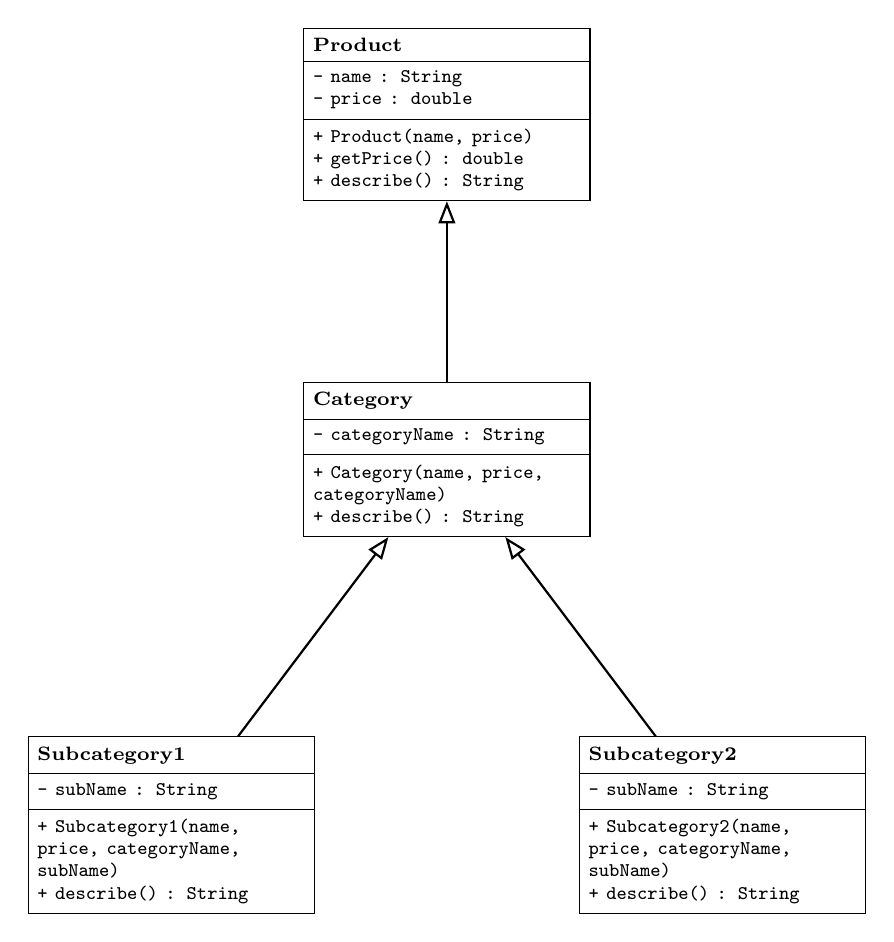
\begin{tikzpicture}
    \umlclass{Product}
             {\texttt{- name : String}\\ \texttt{- price : double}}
             {\texttt{+ Product(name, price)}\\ \texttt{+ getPrice() : double}\\ \texttt{+ describe() : String}}
             {0}{0}
    \umlclass{Category}
             {\texttt{- categoryName : String}}
             {\texttt{+ Category(name, price, categoryName)}\\ \texttt{+ describe() : String}}
             {0}{-4.5}
    \umlclass{Subcategory1}
             {\texttt{- subName : String}}
             {\texttt{+ Subcategory1(name, price, categoryName, subName)}\\ \texttt{+ describe() : String}}
             {-3.5}{-9}
    \umlclass{Subcategory2}
             {\texttt{- subName : String}}
             {\texttt{+ Subcategory2(name, price, categoryName, subName)}\\ \texttt{+ describe() : String}}
             {3.5}{-9}
    \draw[inherits] (Category) -- (Product);
    \draw[inherits] (Subcategory1) -- (Category);
    \draw[inherits] (Subcategory2) -- (Category);
\end{tikzpicture}
\end{center}

\subquestion{a}{6}
Implement \texttt{Product}, \texttt{Category}, \texttt{Subcategory1} and
\texttt{Subcategory2} exactly as shown in the diagram. Every subclass must
call its parent constructor with \texttt{super(...)} and override
\texttt{describe()} so that it appends its own field to the parent's
description.

\subquestion{b}{4}
Write a \texttt{main} method that creates one object of each class, stores
all four in a \texttt{Product[]} array, and prints the result of
\texttt{describe()} for each element. The expected console output is shown
below.

\begin{expectedoutput}
> Pen (price: 5.0)\\
> Pen (price: 5.0) | Category: Stationery\\
> Pen (price: 5.0) | Category: Stationery | Sub: Writing\\
> Pen (price: 5.0) | Category: Stationery | Sub: Packing
\end{expectedoutput}


\end{document}